\chapter{Validação}

Com o objetivo de validar o modelo proposto, é realizada uma pesquisa comparativa com foco no impacto em relação ao uso da ferramenta implementada e mudanças no fluxo de dados sobre APIs Web. Para isso, é desenvolvido um ambiente de validação onde dois clientes, um com a ferramenta e o outro não, realizam três consultas na API de um serviço REST. Por fim, é aplicada uma série de quatro mudanças no fluxo de dados da API e coletados os dados para análise do impacto causado no código de busca desses clientes. \\

\textbf{Escopo de serviço} \\

Foi escolhido trabalhar com um escopo de serviço conhecido como SWAPI (\textit{Starwars API}), bastante utilizado para análise de implementações de tecnologias e estilos de arquitetura em linguagens de programação. Nele, são descritos seis entidades (Pessoa, Filme, Espaçonave, Veículo, Espécie, Planeta) e seus respectivos relacionamentos. Dentro do escopo de serviço, é implementado uma API REST que expõe consultas dessas entidades em formato JSON através de pontos de acesso em URIs, visto na tabela 6. Nota-se que as representações possuem apenas um nível de expansão, ou seja, para acesso dos relacionamentos é preciso consultar a API através de links descritos pela estrutura de retorno (HATEOAS).

\begin{table}[H]
  \centering
  \begin{tabular}{|l|c|}
    \hline
    URI & Descrição \\
    \hline
    /people & Busca lista de pessoas \\
    \hline
    /people/:id & Busca pessoa pelo id \\
    \hline
    /films & Busca lista de filmes \\
    \hline
    /films/:id & Busca filme pelo id \\
    \hline
    /starships & Busca lista de espaçonaves \\
    \hline
    /starships/:id & Busca espaçonave pelo id \\
    \hline
    /vehicles & Busca lista de veículos \\
    \hline
    /vehicles/:id & Busca veículo pelo id \\
    \hline
    /species & Busca lista de espécies \\
    \hline
    /species/:id & Busca espécie pelo id \\
    \hline
    /planets & Busca lista de planetas \\
    \hline
    /planets/:id & Busca planeta pelo id \\
    \hline
  \end{tabular}
  \caption{Pontos de acesso (GET) SWAPI}
\end{table}

\textbf{Perguntas e respostas esperadas} \\

Com o propósito de explorar cada ponto de acesso para busca de dados na SWAPI, foram determinadas três perguntas de média complexidade, onde fossem envolvidos ao menos três das entidades do escopo. Para cada pergunta existe apenas uma resposta certa, onde sua lógica é baseada em campos das estruturas de dados de retorno.

\begin{enumerate}
\item[\textbf{Q1.}] Qual o nome do filme no qual aparecem mais personagens oriundos de um planeta deserto? \textbf{R:} "Revenge of the Sith"
\item[\textbf{Q2.}] Qual o nome da espécie predominante entre os habitantes do planeta "Tatooine"? \textbf{R:} "Droid"
\item[\textbf{Q3.}] Qual o nome do personagem que mais pilota espaçonaves e veículos durante o filme "A New Hope"? \textbf{R:} "Chewbacca"
\end{enumerate}

No intuito de atingir as respostas esperadas, a tabela 7 descreve o fluxo de dados necessário de cada pergunta para a busca de dados por clientes.

\begin{table}[H]
  \centering
  \begin{tabular}{|c|c|c|}
    \hline
    Pergunta & Fluxo de Dados & Número de requisições \\
    \hline
    Q1 & \begin{minipage}[t]{0.3\textwidth}
      \begin{itemize}
        \item[\textbf{GET}] /api/films
        \item[\textbf{GET}] /api/people/:id
        \item[\textbf{GET}] /api/planet/:id
      \end{itemize}
    \end{minipage} & \begin{minipage}[t]{0.5\textwidth}
      \begin{itemize}
        \item[\textbf{x1}] films
        \item[\textbf{x162}] films.characters
        \item[\textbf{x162}] films.characters.homeworld
      \end{itemize}
    \end{minipage} \\
    \hline
    Q2 & \begin{minipage}[t]{0.3\textwidth}
      \begin{itemize}
        \item[\textbf{GET}] /api/planets/1
        \item[\textbf{GET}] /api/people/:id
        \item[\textbf{GET}] /api/species/:id
      \end{itemize}
    \end{minipage} & \begin{minipage}[t]{0.5\textwidth}
      \begin{itemize}
        \item[\textbf{x1}] planet
        \item[\textbf{x10}] planet.residents
        \item[\textbf{x2}] planet.residents.species
      \end{itemize}
    \end{minipage} \\
    \hline
    Q3 & \begin{minipage}[t]{0.3\textwidth}
      \begin{itemize}
        \item[\textbf{GET}] /api/films/1
        \item[\textbf{GET}] /api/starships/:id
        \item[\textbf{GET}] /api/people/:id
        \item[\textbf{GET}] /api/vehicles/:id
        \item[\textbf{GET}] /api/people/:id
      \end{itemize}
    \end{minipage} & \begin{minipage}[t]{0.5\textwidth}
      \begin{itemize}
        \item[\textbf{x1}] film
        \item[\textbf{x8}] film.starships
        \item[\textbf{x9}] film.starships.pilots
        \item[\textbf{x4}] film.vehicles
        \item[\textbf{x0}] film.vehicles.pilots
      \end{itemize}
    \end{minipage} \\
    \hline
  \end{tabular}
  \caption{Fluxo de dados para responder as perguntas}
\end{table}

\textbf{Consultas e metadados} \\

Para permitir a comunicação entre o cliente que faz o uso da ferramenta com a SWAPI, foi preciso implementar três consultas GraphQL (uma para cada pergunta), além de descrever os metadados da API REST. Nas consultas da figura 26, foram realizadas apenas a busca de dados necessários para o funcionamento da lógica de resposta. Enquanto aos metadados da figura 27, foram descritos apenas os pontos de acesso utilizados no formato JSON Hyper-Schema, junto com implementação de um adaptador para a ferramenta que consiga interpretar este formato.

\begin{figure}[H]
  \centering
  \begin{minted}[frame=single,framesep=10pt,fontsize=\footnotesize]{text}
      query q1 {
        allFilms {
          title
          characters {
            homeworld {
              climate
            }
          }
        }
      }

      query q2 {
        planet(planetID: 1) {
          residents {
            species {
              name
            }
          }
        }
      }

      query q3 {
        film(filmID: 1) {
          starships {
            pilots {
              name
            }
          }
          vehicles {
            pilots {
              name
            }
          }
        }
      }
  \end{minted}
  \caption{Consultas GraphQL para as perguntas}
\end{figure}

\begin{figure}[H]
  \centering
  \begin{minted}[frame=single,framesep=10pt,fontsize=\footnotesize]{text}
    {
      "$schema": "http://json-schema.org/draft-04/hyper-schema#",
      "title": "swapi",
      "type": "object",
      "definitions": {
        "allFilms": { ... },
        "film": { ... },
        "people": { ... },
        "planet": { ... },
        "species": { ... },
        "starship": { ... },
        "vehicle": { ... }
      },
      "properties": {
        "allFilms": { "$ref": "#/definitions/allFilms" },
        "film": { "$ref": "#/definitions/film" },
        "people": { "$ref": "#/definitions/people" },
        "planet": { "$ref": "#/definitions/planet" },
        "species": { "$ref": "#/definitions/species" },
        "starship": { "$ref": "#/definitions/starship" }
      },
      "links": [{
        "rel": "allFilms",
        "href": "/films",
        "targetSchema": {
          "$ref": "#/definitions/allFilms"
        }
      }, {
        "rel": "film",
        "href": "/films/{filmID}",
        "schema": { ... },
        "targetSchema": {
          "$ref": "#/definitions/film"
        }
      }, {
        "rel": "planet",
        "href": "/planets/{planetID}",
        "schema": { ... },
        "targetSchema": {
          "$ref": "#/definitions/planet"
        }
      }]
    }
  \end{minted}
  \caption{JSON Hyper-Schema para SWAPI}
\end{figure}

\textbf{Mudanças no fluxo de dados} \\

Para avaliar o impacto no código em ambos clientes, é proposto quatro tipos de mudanças na API não acumulativas que afetam o fluxo de dados. Cada uma busca testar a capacidade da ferramenta em se adaptar e realizar a comunicação mesmo após a alteração no fluxo. Nota-se que, para cada mudança na API do serviço, é preciso a atualização de seus metadados para a correta operação da ferramenta. A tabela 8 descreve o changelog das mudanças realizadas.

\begin{table}[H]
  \centering
  \begin{tabular}{|c|c|c|}
    \hline
    Mudança & Descrição & Changelog \\
    \hline
    C1 & \begin{minipage}[t]{0.3\textwidth}
      Mudança no endereço de ponto de acesso.
    \end{minipage} & \begin{minipage}[t]{0.5\textwidth}
      \begin{itemize}
        \item Renomeação da URI /films para /movies.
        \item Renomeação da URI /films/:id para /movies/:id
      \end{itemize}
    \end{minipage} \\
    \hline
    C2 & \begin{minipage}[t]{0.3\textwidth}
      Mudança no nível de estrutura de resposta.
    \end{minipage} & \begin{minipage}[t]{0.5\textwidth}
      \begin{itemize}
        \item Expansão do campo pilots da URI /starships/:id
        \item Expansão do campo pilots da URI /vehicles/:id
      \end{itemize}
    \end{minipage} \\
    \hline
    C3 & \begin{minipage}[t]{0.3\textwidth}
      Adição de ponto de acesso otimizado.
    \end{minipage} & \begin{minipage}[t]{0.5\textwidth}
      \begin{itemize}
        \item[\textbf{+}] Adição da URI /tatooine.
        \item[\textbf{+}] Adição da URI /films/:id/characters.
      \end{itemize}
    \end{minipage} \\
    \hline
    C4 & \begin{minipage}[t]{0.3\textwidth}
      Remoção de ponto de acesso deprecado.
    \end{minipage} & \begin{minipage}[t]{0.5\textwidth}
      \begin{itemize}
        \item[\textbf{+}] Adição da URI /people/:id/homeworld.
        \item[\textbf{$-$}] Remoção da URI /planet/:id.
      \end{itemize}
    \end{minipage} \\
    \hline
  \end{tabular}
  \caption{Changelog do novo fluxo de dado para cada mudança}
\end{table}

\textbf{Variáveis} \\

São descritas cinco variáveis para análise dos quatro testes de validação em cada um dos clientes. Todas são quantitativas e coletadas no cliente após cada processo de mudança da API. Dessa maneira, totalizam um número de 40 dados normalizados possíveis para análise no final da execução nos dois clientes.

\begin{table}[H]
  \centering
  \begin{tabular}{|c|c|c|}
    \hline
    Variável & Unidade & Tipo \\
    \hline
    Porcentagem de acerto & \% & Quantitativa \\
    \hline
    Tamanho de resposta & kb & Quantitativa \\
    \hline
    Número de requisições & inteiro & Quantitativa \\
    \hline
    Tempo de busca de metadados & ms & Quantitativa \\
    \hline
    Tempo de processamento & ms & Quantitativa \\
    \hline
  \end{tabular}
  \caption{Variáveis de coleta e análise}
\end{table}

\section{Resultados}

Os resultados obtidos nos testes de validação apresentam a média dos valores coletados após diversas execuções dos quatro testes de mudança de forma sequencial em uma máquina virtual. Tanto o serviço SWAPI como os clientes JavaScript foram executados no mesmo ambiente computacional, porém com conexão local de latência 10mb/s para simulação de um ambiente distribuído. Para a variável de processamento, foram utilizados valores que pudessem representar um dispositivo computacional de médio porte. (1 CPU de 2.4 GHz e 4gb de RAM)

Inicialmente, observa-se na figura 27 que o cliente 1 (sem o uso da ferramenta) não apresenta um bom índice de acerto das respostas. Dentre as quatro mudanças, obteve apenas 58\% de acerto, sendo a C3 a única mudança em que conseguiu responder certo todas pois não houve mudança nas URIs que estava utilizando. Um resultado esperado, significando que houve quebra de contrato e impacto negativo ao código de busca.

Em contrapartida, o cliente 2 (com o uso da ferramenta) apresenta um resultado no índice de acerto da figura 28 36.61\% superior ao cliente 1. Com um total de 91,5\% de acerto, apenas não completou com 100\% de acerto pois a mudança C4 não permitiu que fosse possível acessar todos os dados necessários para a responder da pergunta Q2. Isso representa que a ferramenta foi capaz, através do intermediador, de evitar a criação de contrato e causar impacto negativo ao código de busca.

Nota-se que ambos os clientes não apresentaram erros na resposta, ao invés acabam não respondendo pois ocorre exceções durante o código de busca ou lógica devido ao impacto das mudanças no fluxo de dados.

\begin{figure}[H]
  \centering
  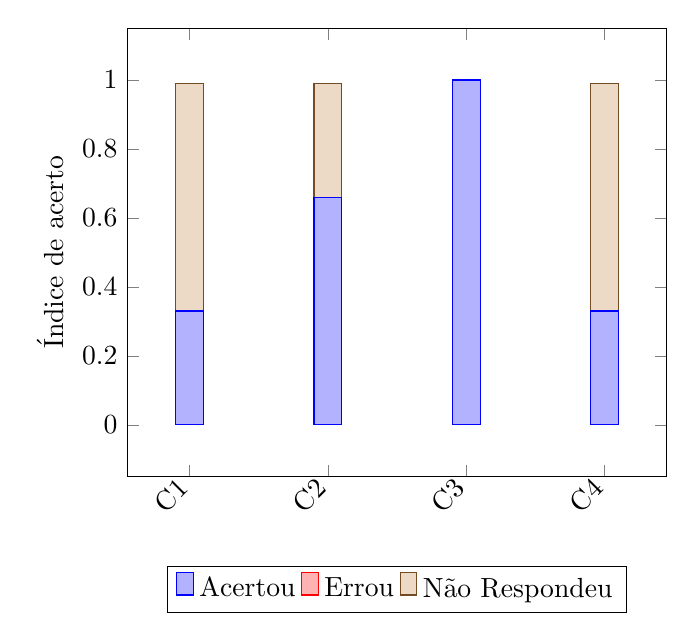
\begin{tikzpicture}
  \begin{axis}[
      ybar stacked,
      ymax=1,
      ymin=0,
      enlargelimits=0.15,
      legend style={at={(0.5,-0.20)},
        anchor=north,legend columns=-1},
      ylabel={Índice de acerto},
      symbolic x coords={C1, C2, C3, C4,
          C5, C6, C7},
      xtick=data,
      x tick label style={rotate=45,anchor=east},
      ]
  \addplot+[ybar] plot coordinates {(C1,0.33) (C2,0.66)
    (C3,1) (C4,0.33)};
  \addplot+[ybar] plot coordinates {(C1,0) (C2,0)
    (C3,0) (C4,0)};
  \addplot+[ybar] plot coordinates {(C1,0.66) (C2,0.33)
    (C3,0) (C4,0.66)};
  \legend{Acertou, Errou, Não Respondeu}
  \end{axis}
  \end{tikzpicture}
  \caption{Índice de acerto sem o uso da ferramenta}
\end{figure}

\begin{figure}[H]
  \centering
  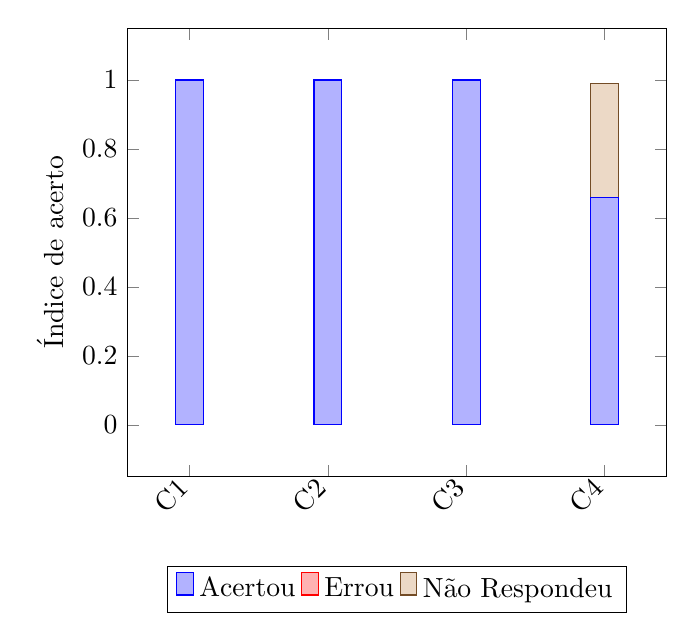
\begin{tikzpicture}
  \begin{axis}[
      ybar stacked,
      ymax=1,
      ymin=0,
      enlargelimits=0.15,
      legend style={at={(0.5,-0.20)},
        anchor=north,legend columns=-1},
      ylabel={Índice de acerto},
      symbolic x coords={C1, C2, C3, C4,
          C5, C6, C7},
      xtick=data,
      x tick label style={rotate=45,anchor=east},
      ]
  \addplot+[ybar] plot coordinates {(C1,1) (C2,1)
    (C3,1) (C4,0.66)};
  \addplot+[ybar] plot coordinates {(C1,0) (C2,0)
    (C3,0) (C4,0)};
  \addplot+[ybar] plot coordinates {(C1,0) (C2,0)
    (C3,0) (C4,0.33)};
  \legend{Acertou, Errou, Não Respondeu}
  \end{axis}
  \end{tikzpicture}
  \caption{Índice de acerto com o uso da ferramenta}
\end{figure}

Ao analisar a mudança C3 isoladamente, onde ambos conseguem responder com 100\% de acerto, percebe-se na figura 29 e 30 que o cliente 2 consegue realizar uma busca mais performática (menor número de requisição e tamanho de dados) que o cliente 1. Isso porque, após a mudança e sem alterar o código de busca de dados, a ferramenta consegue remapear as requisições geradas pelas consultas GraphQL graças ao algoritmo de implementação na automação das chamadas em URIs.

Outro ponto importante é que, após a mudança C3 e atualização dos metadados no cliente, o algoritmo da ferramenta percebe que há a possibilidade de realizar menos requisições em busca dos dados para responder as perguntas. O que resulta em uma redução de aproximadamente 54\% dos acessos entre o cliente 1 e cliente 2.

\begin{figure}[H]
  \centering
  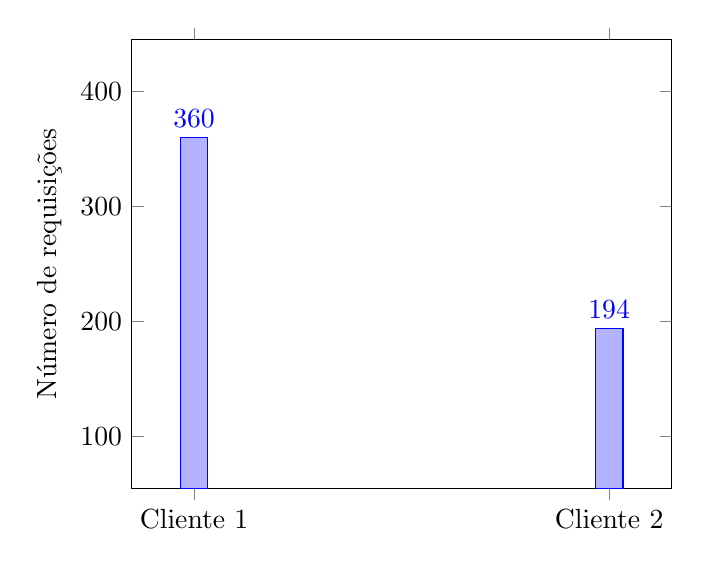
\begin{tikzpicture}
  \begin{axis}[
      ybar,
      ymax=400,
      ymin=100,
      enlargelimits=0.15,
      ylabel={Número de requisições},
      symbolic x coords={Cliente 1,Cliente 2},
      xtick=data,
      nodes near coords,
      nodes near coords align={vertical},
      ]
  \addplot coordinates {(Cliente 1,360) (Cliente 2,194)};
  \end{axis}
  \end{tikzpicture}
  \caption{Comparação no número de requisições C3}
\end{figure}

\begin{figure}[H]
  \centering
  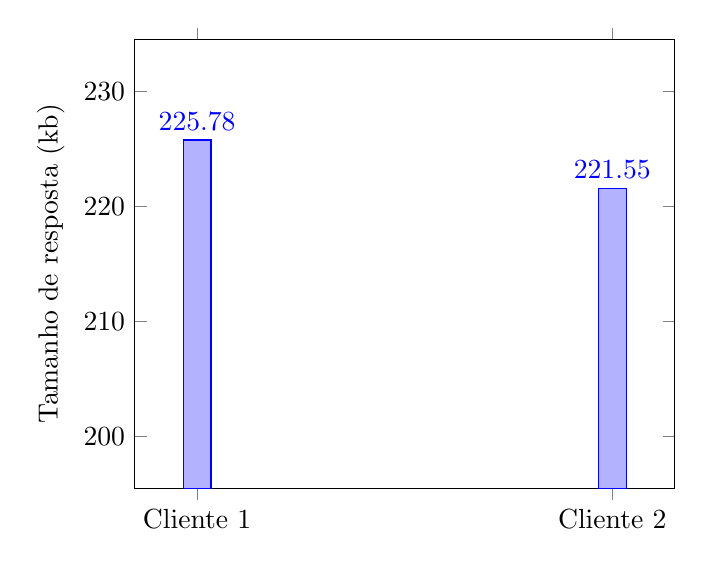
\begin{tikzpicture}
  \begin{axis}[
      ybar,
      ymax=230,
      ymin=200,
      enlargelimits=0.15,
      ylabel={Tamanho de resposta (kb)},
      symbolic x coords={Cliente 1,Cliente 2},
      xtick=data,
      nodes near coords,
      nodes near coords align={vertical},
      ]
  \addplot coordinates {(Cliente 1,225.777) (Cliente 2,221.547)};
  \end{axis}
  \end{tikzpicture}
  \caption{Comparação no tamanho de resposta C3}
\end{figure}

Apesar dos ganhos de performance e desenvolvimento através do uso da ferramenta vistos anteriormente, percebe-se na figura 31 um outro cenário em que indica o lado negativo do seu uso causado pelo tempo de \textit{overhead}\footnote{
  Processamento em excesso
}. Em média, a ferramenta atrasou em 1.7 segundos a execução na consulta de dados do cliente, sendo o tempo de busca de metadados responsável por somar mais da metade deste atraso inicial.

Contudo, é importante levar em conta que este tempo de \textit{overhead} é um impasse da ferramenta, mas também relativo ao tempo de vida do cliente que está sendo executado. Por exemplo, em clientes com tempo de vida curto ou que dependem de carregamento rápido, a ferramenta pode não ser a solução ideal. Nos demais casos, é visível os benefícios que seu uso pode trazer.

\begin{figure}[H]
  \centering
  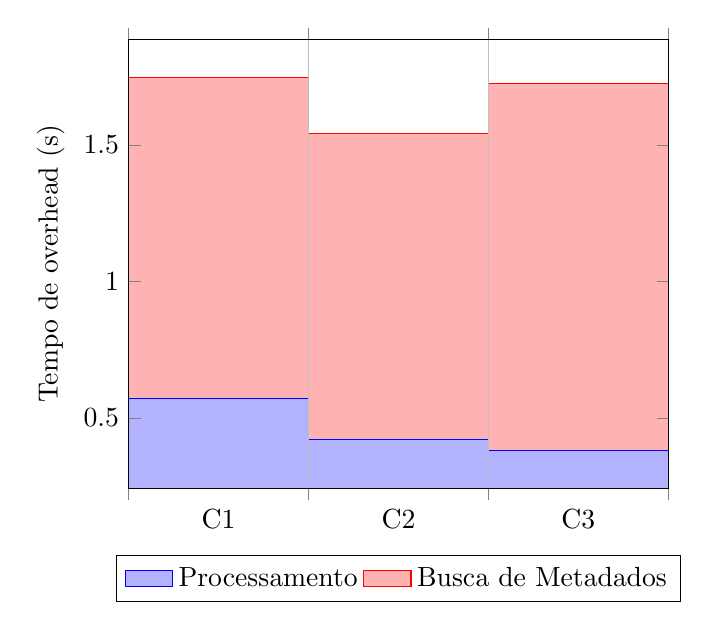
\begin{tikzpicture}
	\begin{axis}[
        ybar interval,
        ylabel={Tempo de overhead (s)},
        legend style={at={(0.5,-0.15)},
        anchor=north,legend columns=-1},
        const plot,
		stack plots=y,
		area style,
        symbolic x coords={C1,C2,C3,C4},
		enlarge x limits=false]
	\addplot coordinates
		{(C1,0.57) (C2,0.42) (C3,0.38) (C4,0.48)}
		\closedcycle;
	\addplot coordinates
		{(C1,1.178) (C2,1.123) (C3,1.343) (C4,1.185)}
		\closedcycle;
    \legend{Processamento,Busca de Metadados}
	\end{axis}
  \end{tikzpicture}
  \caption{Overhead da ferramenta}
\end{figure}

